\documentclass[12pt]{article}

\usepackage{amsmath}
\usepackage{amssymb}
\usepackage{amsthm}

\usepackage{algorithm}
\usepackage{algorithmic}

\usepackage{geometry}

\usepackage{tikz}
\usetikzlibrary{arrows}

\title{CS420 - Homework \#1}
\author{Trevor Bramwell}
\date{February 6, 2014}

\begin{document}
\maketitle

\section*{Problem 1}

Throughout the lecture, we assumed that no two edges in the input graph
have equal weights, which implies that the minimum spanning tree is
unique. In fact, a weaker condition on the edge weights implies MST
uniqueness.

\subsection*{(a)}
Describe an edge-weighted graph that has a unique minimum spanning tree,
even though two edges have equal weights.

\begin{center}
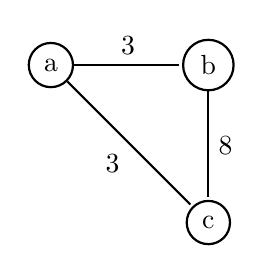
\begin{tikzpicture}[-,>=stealth',shorten >=1pt,auto,node distance=2cm,
                    thick]
  \tikzstyle{every state}=[fill=white]

  \node[draw, circle]   (A)              {a};
  \node[draw, circle]   (B) [right of=A] {b};
  \node[draw, circle]   (C) [below of=B] {c};

  \path (A) edge node {$3$} (B)
            edge [below left] node {$3$} (C)
        (B) edge node {$8$} (C);
\end{tikzpicture}
\end{center}

\subsection*{(b)}
Prove that an edge-weighted graph $G$ has a unique minimum spanning tree
if the following condition holds:

\begin{itemize}
    \item For any partition of the vertices of $G$ into two subsets, the
          minimum-weight edge with one endpoint in each subset is unique.
\end{itemize}

\begin{proof}[Proof by Contradiction]
    Let $G$ be an edge-weighted graph. Let $T_1$, $T_2$ be arbitrary
    partitions of $G$.
    
    Assume the minimum-weight edge with one endpoint in each subset is
    not unique.

    Then $\exists$ some edges $e_1$ and $e_2$ which have one endpoint in each
    subset.

    $\ldots$

\end{proof}

\subsection*{(c)}
Describe and analyze an algorithm to determine whether or not a graph
has a unique minimum spanning tree.

Shimble's algorithm with the minor change that in the second loop:
\begin{algorithm}
\caption{Modified Shimble}
\begin{algorithmic}
  \STATE
  \STATE $\ldots$
  \STATE
  \FOR{every edge $u \rightarrow v$}
    \IF{$u \rightarrow v$ is tense}
      \RETURN False
    \ENDIF
  \RETURN True
  \ENDFOR
\end{algorithmic}
\end{algorithm}


\section*{Problem 2}
Consider the following algorithm for finding the smallest element in an
unsorted array:

\begin{algorithm}
    \caption{RandomMin $A [1 \ldots n]$}
\begin{algorithmic}
  \STATE $min \leftarrow \infty$
  \FOR{$i \leftarrow 1$ to $n$ in random order}
  \IF{ $A [i] < min$ }
  \STATE $min \leftarrow A [i]$ \hspace{1 cm} $(*)$
  \ENDIF
  \ENDFOR
  \RETURN $min$
\end{algorithmic}
\end{algorithm}

\subsection*{(a)}
In the worst case, how many times does RandomMin execute line \(*\)?


\begin{equation*}
O(n)
\end{equation*}

\subsection*{(b)}
What is the probability that line \(*\) is executed during the $n$th
iteration of the for loop?

\begin{equation*}
    \frac{\dbinom{n}{1}}{n!} = \frac{1}{(n-1)!}
\end{equation*}

This states that there are $\binom{n}{1}$ ways to organize the first $n
- 1$ elements of RandomMin out of a total of $n!$ ways the array can be
organized.

\subsection*{(c)}
What is the $exact$ expected number of executions of line \(*\)?


\section*{Problem 3}
The randomized linear time algorithm of Karger, Klein and Tarjan for
finding a minimum spanning tree performs two steps of the Boruvka
algorithm and uses sampling steps in which each edge of the graph is
chosen, independently, with probability 1/2.\newline

The following solutions build off of the equation $\mathbb{E}[T(G)]$
presented by Uri Zwick the Lecture notes for "Analysis of
Algorithms": Minimum Spanning Trees.


\subsection*{(a)}
What would be the running time of the algorithm in terms of $m$, $n$,
and $k$ if it performs $k$ steps of the Boruvka algorithm instead,
where $k$ is a positive integer?

\begin{equation*}
    \mathbb{E}[T(G)] = a(m + n) + 2a(\frac{\bar{m}}{k} + 2 * \frac{\bar{n}}{k^2}) +
    2a(\frac{\bar{n}}{k} + 2 * \frac{\bar{n}}{k^2})
\end{equation*}

\subsection*{(b)}
What would be the expected running time of the algorithm in terms of
$m$, $n$ and $p$ if the sampling probability were changed to $p$ ,
where $0 \le p \le 1$?\\

The sampling probabilty only affects $\bar{m}_1$ in the original equation.
Thus $\bar{m}_1 \le \bar{m}p$

\begin{align*}
    \mathbb{E}[T(G)] &\le a(\bar{m} + \bar{n}) + 2a\left(\bar{m}p
                      + \cdot2\frac{\bar{n}}{4}\right)
                      + 2a(\frac{\bar{n}}{2} + 2\cdot\frac{\bar{n}}{4})\\
                     & \cdots \\
                     &= 2a(\bar{m}(p + 1) + 2\bar{n})
\end{align*}


\pagebreak

\section*{Problem 4}

\subsection*{(a)}
Describe and analyze a modification of Shimbel's shortest-path algorithm
that actually returns a negative cycle if any such cycle is reachable
from $s$, or a shortest-path tree if there is no such cycle. The modified
algorithm should still run in $O(mn)$ time.

\begin{algorithm}
\caption{ShimbleNegCycleOrTree}
\begin{algorithmic}
    \STATE InitSSSP($s$)
    \FORALL{$m$}
        \FORALL{$u \rightarrow v$}
            \IF{$u \rightarrow v$ is tense}
                \STATE Relax($u \rightarrow v$)
            \ENDIF
        \ENDFOR
    \ENDFOR
    \STATE $u_{min} \leftarrow s$
    \FORALL{$u \rightarrow v$}
        \IF{$u \rightarrow v$ is tense}
            \RETURN $\{ recurse\; pred(u)\; until\; v \}$
        \ENDIF
        \IF{$dist(u) < dist(u_{min})$}
            \STATE $u_{min} \leftarrow u$
        \ENDIF
        \RETURN $\{ recurse\; pred(u)\; until\; s \}$
    \ENDFOR
\end{algorithmic}
\end{algorithm}

\pagebreak

\subsection*{(b)}
Describe and analyze a modification of Shimbel's shortest-path
algorithm that computes the correct shortest path distances from $s$ to
every other vertex of the input graph, even if the graph contains
negative cycles. Specifically, if any walk from $s$ to $v$ contains a
negative cycle, your algorithm should end with $dist(v) = -\infty$
otherwise, $dist(v)$ should contain the length of the shortest path
from $s$ to $v$. The modified algorithm should still run in $O(mn)$
time.

\begin{algorithm}
\caption{ShimbleNegativeCycles}
\begin{algorithmic}
    \STATE InitSSSP($s$)
    \FORALL{$m$}
        \FORALL{$u \rightarrow v$}
            \IF{$u \rightarrow v$ is tense}
                \STATE Relax($u \rightarrow v$)
            \ENDIF
        \ENDFOR
    \ENDFOR
    \FORALL{$u \rightarrow v$}
        \IF{$u \rightarrow v$ is tense \OR $dist(u) = -\infty$}
            \STATE $dist(v) = -\infty$
        \ENDIF
    \ENDFOR
\end{algorithmic}
\end{algorithm}

\end{document}
